% !TEX root = Dokumentation_SysSpec.tex
\subsection{Modelle und Sichten}
todo


\subsubsection{Kontextdiagramm}
todo bla
\begin{figure}
	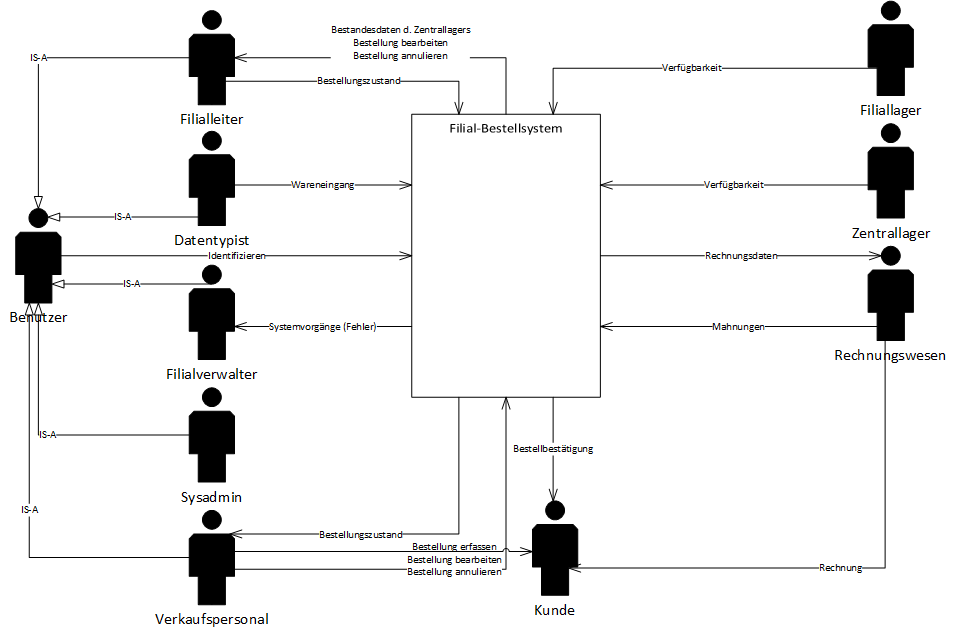
\includegraphics[width=1.0\linewidth]{Images/kontextdiagram}
	\caption{Kontextdiagram}
	\label{fig:kontextdiagram}
\end{figure}


\subsubsection{UML-Klassendiagramme}
todo


\subsubsection{Sequenzdiagramme}
todo


\subsection{Entwurfsentscheid}
Im Rahmen der Architekturausarbeitung wurden folgende Entwurfsentscheide gefällt:
\begin{itemize}
	\item Für Testzwecke und statische Datenstrukturen werden teilweise Stubs eingesetzt. Beispielsweise sind die Zuweisung Benutzerrollen zu deren Berechtigungen bis Release 1.0 als Stub abgebildet.
	\item Der Business-Layer und Data-Layer (ohne Datenbank, nur OR-Mapper) befinden sich auf dem gleichen Tier. Bis Release 1.0 werden, aus zeitlichen Gründen, keine Bestrebungen zur Aufteilung dieser Layers auf verschiedene Tiers vorgenommen
	\item Die Tier-übergreifende Kommunikation zwischen Tier Client und Business wird mittels RMI (Remote Method Invocation) umgesetzt. Eine alternative Anbindung bspw. mit REST (Representational state transfer) wird nach Release 1.0 in Betracht gezogen.
	\item Als GUI-Komponente auf Layer Client wird JavaFX verwendet.
	\item Als Datenbank wird eine MySQL-Instanz aus dem EnterpriseLab der HSLU verwendet.
	\item Bis Release 1.0 müssen neue Kunden \& Artikel in der Datenbank manuell erfasst / abgebildet werden.
	\item Die Rechnungsdaten und Mahnungen werden aufgrund der 
\end{itemize}


TODO
- Dateien einbinden (DB) -> Transaktionsmanagement

